%\documentclass{beamer}
\documentclass[xcolor=dvipsnames]{beamer}
\usepackage[latin1]{inputenc}
\usepackage{hyperref}
\usecolortheme[named=Violet]{structure}
\usetheme{Warsaw}
\usepackage{listings}
\usepackage{color}
\usepackage{simpsons}

\definecolor{dkgreen}{rgb}{0,0.6,0}
\definecolor{gray}{rgb}{0.5,0.5,0.5}
\definecolor{mauve}{rgb}{0.58,0,0.82}

% "define" julia
\lstdefinelanguage{julia}{morekeywords={function,if,else,while,for,:,end}, sensitive=true, morecomment=[l]{\#}, morecomment=[s]{/*}{*/}, morestring=[b]"}

% Default settings for code listings
\lstset{frame=tb,
   language=julia,
   aboveskip=3mm,
   belowskip=3mm,
   showstringspaces=false,
   columns=flexible,
   basicstyle={\small\ttfamily},
   numbers=none,
   frame=none,
   numberstyle=\tiny\color{gray},
   keywordstyle=\color{blue},
   commentstyle=\color{dkgreen},
   stringstyle=\color{mauve},
   breaklines=true,
   breakatwhitespace=true
   tabsize=3
}

\title[Scientific Computing]{Elements of Scientific Computing with Julia}
\begin{document}

\begin{frame}
\titlepage
\end{frame}

\AtBeginSubsection[]
{
  \begin{frame}<beamer>
    \frametitle{Today's Class}
    \tableofcontents[currentsection,currentsubsection]
  \end{frame}
}
\section{Programming with Julia}
\begin{frame}[fragile]
{\bf Nice to meet you, Julia!}
Julia is a high-level, high-performance, dynamic programming language. This means that you can spend more time worrying about your scientific computing problems and models, rather than providing detailed computer instructions in your code.
\vfill
\pause
\begin{enumerate}
\item Julia is free and open source;\pause
\item Unlike MATLAB, de-vectorized code is fast;\pause
\item Julia is well equipped for parallel computing;\pause
\item We can call C functions directly;\pause
\item Power type system - support for arbitrary precision.
\end{enumerate}
\end{frame}

\begin{frame}[fragile]
{\bf Julia: A Crash Course}
\begin{lstlisting}
# There are several basic types of numbers.
3 #=> 3 (Int64)
3.2 #=> 3.2 (Float64)
2 + 1im #=> 2 + 1im (Complex{Int64})
2//3 #=> 2//3 (Rational{Int64})

# All of the normal infix operators are available.
1 + 1 #=> 2
8 - 1 #=> 7
10 * 2 #=> 20
35 / 5 #=> 7.0
5 / 2 #=> 2.5 # dividing an Int by an Int always results in a Float
div(5, 2) #=> 2 # for a truncated result, use div
5 \ 35 #=> 7.0
2 ^ 2 #=> 4 # power, not bitwise xor
12 % 10 #=> 2
\end{lstlisting}
\end{frame}

\begin{frame}[fragile]
{\bf Julia: A Crash Course}
\begin{lstlisting}
# Boolean operators
!true #=> false
!false #=> true
1 == 1 #=> true
2 == 1 #=> false
1 != 1 #=> false
2 != 1 #=> true
1 < 10 #=> true
1 > 10 #=> false
2 <= 2 #=> true
2 >= 2 #=> true

# Comparisons can be chained
1 < 2 < 3 #=> true
2 < 3 < 2 #=> false
\end{lstlisting}
\end{frame}

\begin{frame}[fragile]
{\bf Julia: A Crash Course}
\begin{lstlisting}
# Strings are created with "
"This is a string."
# Character literals are written with '
'a'
# A string can be indexed like an array of characters
"This is a string"[1] #=> 'T' # Julia indexes from 1

# $ can be used for string interpolation:
"2 + 2 = $(2 + 2)" #=> "2 + 2 = 4"
# You can put any Julia expression inside the parenthesis.

# Another way to format strings is the printf macro.
@printf "%d is less than %f" 4.5 5.3 # 5 is less than 5.300000

# Printing is easy
println("I'm Julia. Nice to meet you!")
\end{lstlisting}
\end{frame}

\begin{frame}[fragile]
{\bf Julia: A Crash Course}
\begin{lstlisting}
# Arrays store a sequence of values indexed by integers 1 through n:
a = Int64[] #=> 0-element Int64 Array

# Note that arrays must be given a type, and all elements in the array must be of that type.

# 1-dimensional array literals can be written with comma-separated values.
b = [4, 5, 6] #=> 3-element Int64 Array: [4, 5, 6]
b[1] #=> 4
b[end] #=> 6

# 2-dimentional arrays use space-separated values and semicolon-separated rows.
matrix = [1 2; 3 4] #=> 2x2 Int64 Array: [1 2; 3 4]
\end{lstlisting}
\end{frame}

\begin{frame}[fragile]
{\bf Julia: A Crash Course}
\begin{lstlisting}
# Add stuff to the end of an array with push! and append!
push!(a,1)     #=> [1]
push!(a,2)     #=> [1,2]
push!(a,4)     #=> [1,2,4]
push!(a,3)     #=> [1,2,4,3]
append!(a,b) #=> [1,2,4,3,4,5,6]

# Remove from the end with pop
pop!(b)        #=> 6 and b is now [4,5]

# Let's put it back
push!(b,6)   # b is now [4,5,6] again.

a[1] #=> 1 # remember that Julia indexes from 1, not 0!
\end{lstlisting}
\end{frame}

\begin{frame}[fragile]
{\bf Julia: A Crash Course}
\begin{lstlisting}
# Function names that end in exclamations points indicate that they modify their argument.
arr = [5,4,6] #=> 3-element Int64 Array: [5,4,6]
sort(arr) #=> [4,5,6]; arr is still [5,4,6]
sort!(arr) #=> [4,5,6]; arr is now [4,5,6]

# You can initialize arrays from ranges
a = [1:5] #=> 5-element Int64 Array: [1,2,3,4,5]

# You can look at ranges with slice syntax.
a[1:3] #=> [1, 2, 3]
a[2:] #=> [2, 3, 4, 5]
a[2:end] #=> [2, 3, 4, 5]
\end{lstlisting}
\end{frame}

\begin{frame}[fragile]
{\bf Julia: A Crash Course}
\begin{lstlisting}
# Remove elements from an array by index with splice!
arr = [3,4,5]
splice!(arr,2) #=> 4 ; arr is now [3,5]

# Check for existence in an array with in
in(1, a) #=> true

# Examine the length with length
length(a) #=> 8
\end{lstlisting}
\end{frame}

\begin{frame}[fragile]
{\bf Julia: A Crash Course}
\begin{lstlisting}
# Tuples are immutable.
tup = (1, 2, 3) #=> (1,2,3) # an (Int64,Int64,Int64) tuple.
tup[1] #=> 1

# Many array functions also work on tuples
length(tup) #=> 3
tup[1:2] #=> (1,2)
in(2, tup) #=> true

# Tuples are created even if you leave out the parentheses
d, e, f = 4, 5, 6 #=> (4,5,6)

# Look how easy it is to swap two values
e, d = d, e  #=> (5,4) # d is now 5 and e is now 4
\end{lstlisting}
\end{frame}

\begin{frame}[fragile]
{\bf Julia: A Crash Course}
\begin{lstlisting}
# Dictionaries store mappings
empty_dict = Dict() #=> Dict{Any,Any}()

# You can create a dictionary using a literal
filled_dict = ["one"=> 1, "two"=> 2, "three"=> 3]

# Look up values with []
filled_dict["one"] #=> 1

# Get all keys
keys(filled_dict)
# Get all values
values(filled_dict)

# Check for existence in a dictionary with in or haskey
in(("two", 3), filled_dict) #=> false
haskey(filled_dict, "one") #=> true
\end{lstlisting}
\end{frame}

\begin{frame}[fragile]
{\bf Julia: A Crash Course}
\begin{lstlisting}
# Here is an if statement. Indentation is not meaningful in Julia, but it is good for readability.

if some_var > 10
    println("some_var is totally bigger than 10.")
elseif some_var < 10    # This elseif clause is optional.
    println("some_var is smaller than 10.")
else                    # The else clause is optional too.
    println("some_var is indeed 10.")
end
#=> prints "some var is smaller than 10"
\end{lstlisting}
\end{frame}

\begin{frame}[fragile]
{\bf Julia: A Crash Course}
\begin{lstlisting}
# For loops iterate over iterables.
# Iterable types include Range, Array, Set, Dict, and String.
for animal=["dog", "cat", "mouse"]
    println("$animal is a mammal")
    # You can use $ to interpolate variables or expression into strings
end
# prints:
#    dog is a mammal
#    cat is a mammal
#    mouse is a mammal

# You can use 'in' instead of '='.
for animal in ["dog", "cat", "mouse"]
    println("$animal is a mammal")
end
\end{lstlisting}
\end{frame}

\begin{frame}[fragile]
{\bf Julia: A Crash Course}
\begin{lstlisting}
# While loops loop while a condition is true
x = 0
while x < 4
    println(x)
    x += 1  # Shorthand for x = x + 1
end
# prints:
#   0
#   1
#   2
#   3

# Handle exceptions with a try/catch block
try
   error("help")
catch e
   println("caught it $e")
end
#=> caught it ErrorException("help")
\end{lstlisting}
\end{frame}

\begin{frame}[fragile]
{\bf Julia: A Crash Course}
\begin{lstlisting}
# The keyword 'function' creates new functions
#function name(arglist)
#  body...
#end
function add(x, y)
    println("x is $x and y is $y")

    # Functions return the value of their last statement
    x + y
end

add(5, 6) #=> 11 after printing out "x is 5 and y is 6"
\end{lstlisting}
\end{frame}

\begin{frame}[fragile]
{\bf Julia: A Crash Course}
\begin{lstlisting}
# You can define functions with optional positional arguments
function defaults(a,b,x=5,y=6)
    return "$a $b and $x $y"
end

defaults('h','g') #=> "h g and 5 6"
defaults('h','g','j') #=> "h g and j 6"
defaults('h','g','j','k') #=> "h g and j k"
try
    defaults('h') #=> ERROR: no method defaults(Char,)
    defaults() #=> ERROR: no methods defaults()
catch e
    println(e)
end
\end{lstlisting}
\end{frame}

\begin{frame}[fragile]
{\bf Julia: A Crash Course}
\begin{lstlisting}
# Julia supports functional programming - stuff like currying and higher order functions
function create_adder(x)
    function adder(y)
        x + y
    end
    adder
end

add_10 = create_adder(10)
add_10(3) #=> 13

# There are built-in higher order functions
map(add_10, [1,2,3]) #=> [11, 12, 13]
filter(x -> x > 5, [3, 4, 5, 6, 7]) #=> [6, 7]
\end{lstlisting}
\end{frame}

\begin{frame}[fragile]
{\bf Arbitrary Precision Arithmetic}
One thing worth emphasizing is Julia's capabilities for arbitrary precision arithmetic. Recall the example we worked on in Lecture 1: 
\vfill
\pause

Write a Julia program to compute the mathematical constant e, the base of natural logarithms, from the definition:
\[ e = \lim\limits_{n \rightarrow \infty} (1+1/n)^n \]
Compute $(1 + 1/n)^n$ for $n = 10^k$, $k = 1, 2, ..., 20$ and determine the error in the successive approximations by comparing them with the value of the built in constant $e$.  \\
\end{frame}

\begin{frame}[fragile]
{\bf Arbitrary Precision Arithmetic}
If we enter the following \emph{modified} code into IJulia:
\begin{lstlisting}
for k = 1:2:20
    a = (1+BigFloat(1/10^k))^BigFloat(10^k)
    err = a - e
    @printf("For k = %d, we get the approximation: %1.12f and the error %1.12f \n", 
    k, a, err)
end
\end{lstlisting}
\end{frame}

\begin{frame}[fragile]
{\bf Arbitrary Precision Arithmetic}
We get the following output:
\begin{verbatim}
For k = 1,  we get the approximation: 2.593742460100 and 
the error -0.124539368359045110601357 
For k = 3,  we get the approximation: 2.716923932236 and 
the error -0.001357896223152721491140 
...
For k = 15, we get the approximation: 2.718281828459 and 
the error -0.000000000000001147915738 
For k = 17, we get the approximation: 2.718281828459 and 
the error  0.000000000000000180881062 
For k = 19, we get the approximation: 2.718281828459 and 
the error -0.000000000000000253747066
\end{verbatim}
\end{frame}

\section{Numerical Integration: Concepts}
\begin{frame}[fragile]
{\bf But my calc teacher said not to use a computer...}
In Calc II class, you probably learned many different ways for algebraically solving for the definite integral of different functions. You were able to apply the Fundamental Theorem of Calculus to definite integrals and you got an exact answer. 
\vfill \pause 
However, you may have come across interesting integrable functions whose antiderivatives were difficult or even impossible to write, such as the famous probability density function for the normal distribution: $f(x)= \displaystyle \frac{1}{\sqrt{2 \pi}}e^{-x^2/2}$. 
\vfill \pause
In this lecture we will look at quadrature methods for solving one dimensional definite integrals numerically.\\
\end{frame}

\begin{frame}[fragile]
{\bf Quadrature Methods}
Quadrature means to calculate the area, and as you may recall, the definite integral of a function can be interpreted as the area under the graph of the function within a particular interval. \vfill \pause We can chop up the area of an unfamiliar shape into slices, and approximate the area of each slice with the area of a familiar shape (such as a rectangle or a trapezoid). \vfill \pause 
If we add up the area of all these slices, we should get an approximation of the are under the given curve, and thus the approximate solution of the definite integral of the given function.\\
\end{frame}

\begin{frame}[fragile]
{\bf Rules, rules, rules!}
For all of the rules below consider the definite integral $\int\limits_a^b f(x) dx$, that is, the area under the curve $f$ in the closed interval $[a, b]$. We divide $[a, b]$ into $n$ subintervals of equal width $\Delta x = \frac{b - a}{n}$. \\
\end{frame}

\begin{frame}[fragile]
{\bf Midpoint Rule}
This rule obtains the area under the curve by subdividing the area into rectangles of equal width $\Delta x$ and height $f(x^*_i)$, where $x^*_i$ is the {\bf midpoint} of the subinterval $[x_{i-1}, x_i]$. 
\vfill \pause
The area of each rectangle is then  $\displaystyle\Delta x f(x^*_i)$, and therefore, we get that:
\[ \int\limits_a^b f(x) dx \approx \Delta x f(x^*_1) + \Delta x f(x^*_2) + ... + \Delta x f(x^*_n)\]
\begin{center}
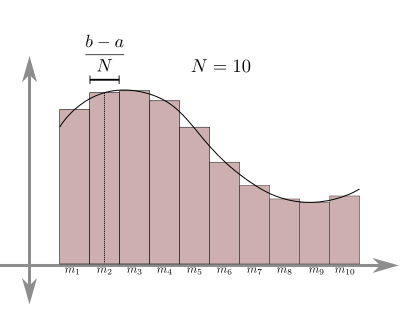
\includegraphics[width=1.5in]{MidpointRule.png}
\end{center}
\end{frame}

\begin{frame}[fragile]
{\bf Trapezoidal Rule}
This rule obtains the area under the curve by subdividing the area into trapezoids of equal trapezoidal height $\Delta x$, and base widths $f(x_{i-1})$ and $f(x_i)$ for each subinterval $[x_{i-1}, x_i]$. 
\vfill \pause
The area of each trapezoid is then $\displaystyle\frac{\Delta x}{2}(f(x_{i-1}) + f(x_i))$, and therefore, we get that:
$\int\limits_a^b f(x) dx \approx $ 
\[\frac{\Delta x}{2}(f(x_0) + f(x_1)) + \frac{\Delta x}{2}(f(x_1) + f(x_2)) + ... + \frac{\Delta x}{2}(f(x_{n-1}) + f(x_n))\]
\begin{center}
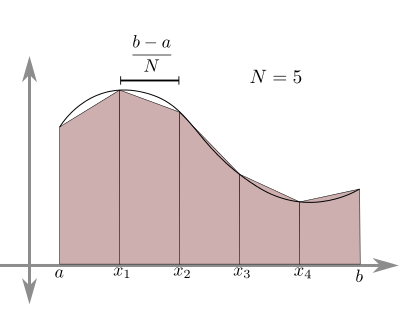
\includegraphics[width=1.5in]{TrapezoidRule.png}
\end{center}
\end{frame}

\begin{frame}[fragile]
{\bf Simpson's Rule}
\Homer - This rule is an interpolative quadrature rule, since upon subdividing the curve into $n = 2k$ (that is, $n$ must be even) slices, we interpolate the best fit quadratic curve for each slice. 
\vfill \pause
If subdivide the interval $[a,b]$ into $n = 2k$ sub-intervals, then we get that: $\int\limits_a^b f(x) dx \approx $ 
\[\frac{\Delta x}{3}[f(x_0) + 4f(x_1) + 2f(x_2) + ... + 2f(x_{n-2}) + 4f(x_{n-1}) + f(x_n)] \]
\begin{center}
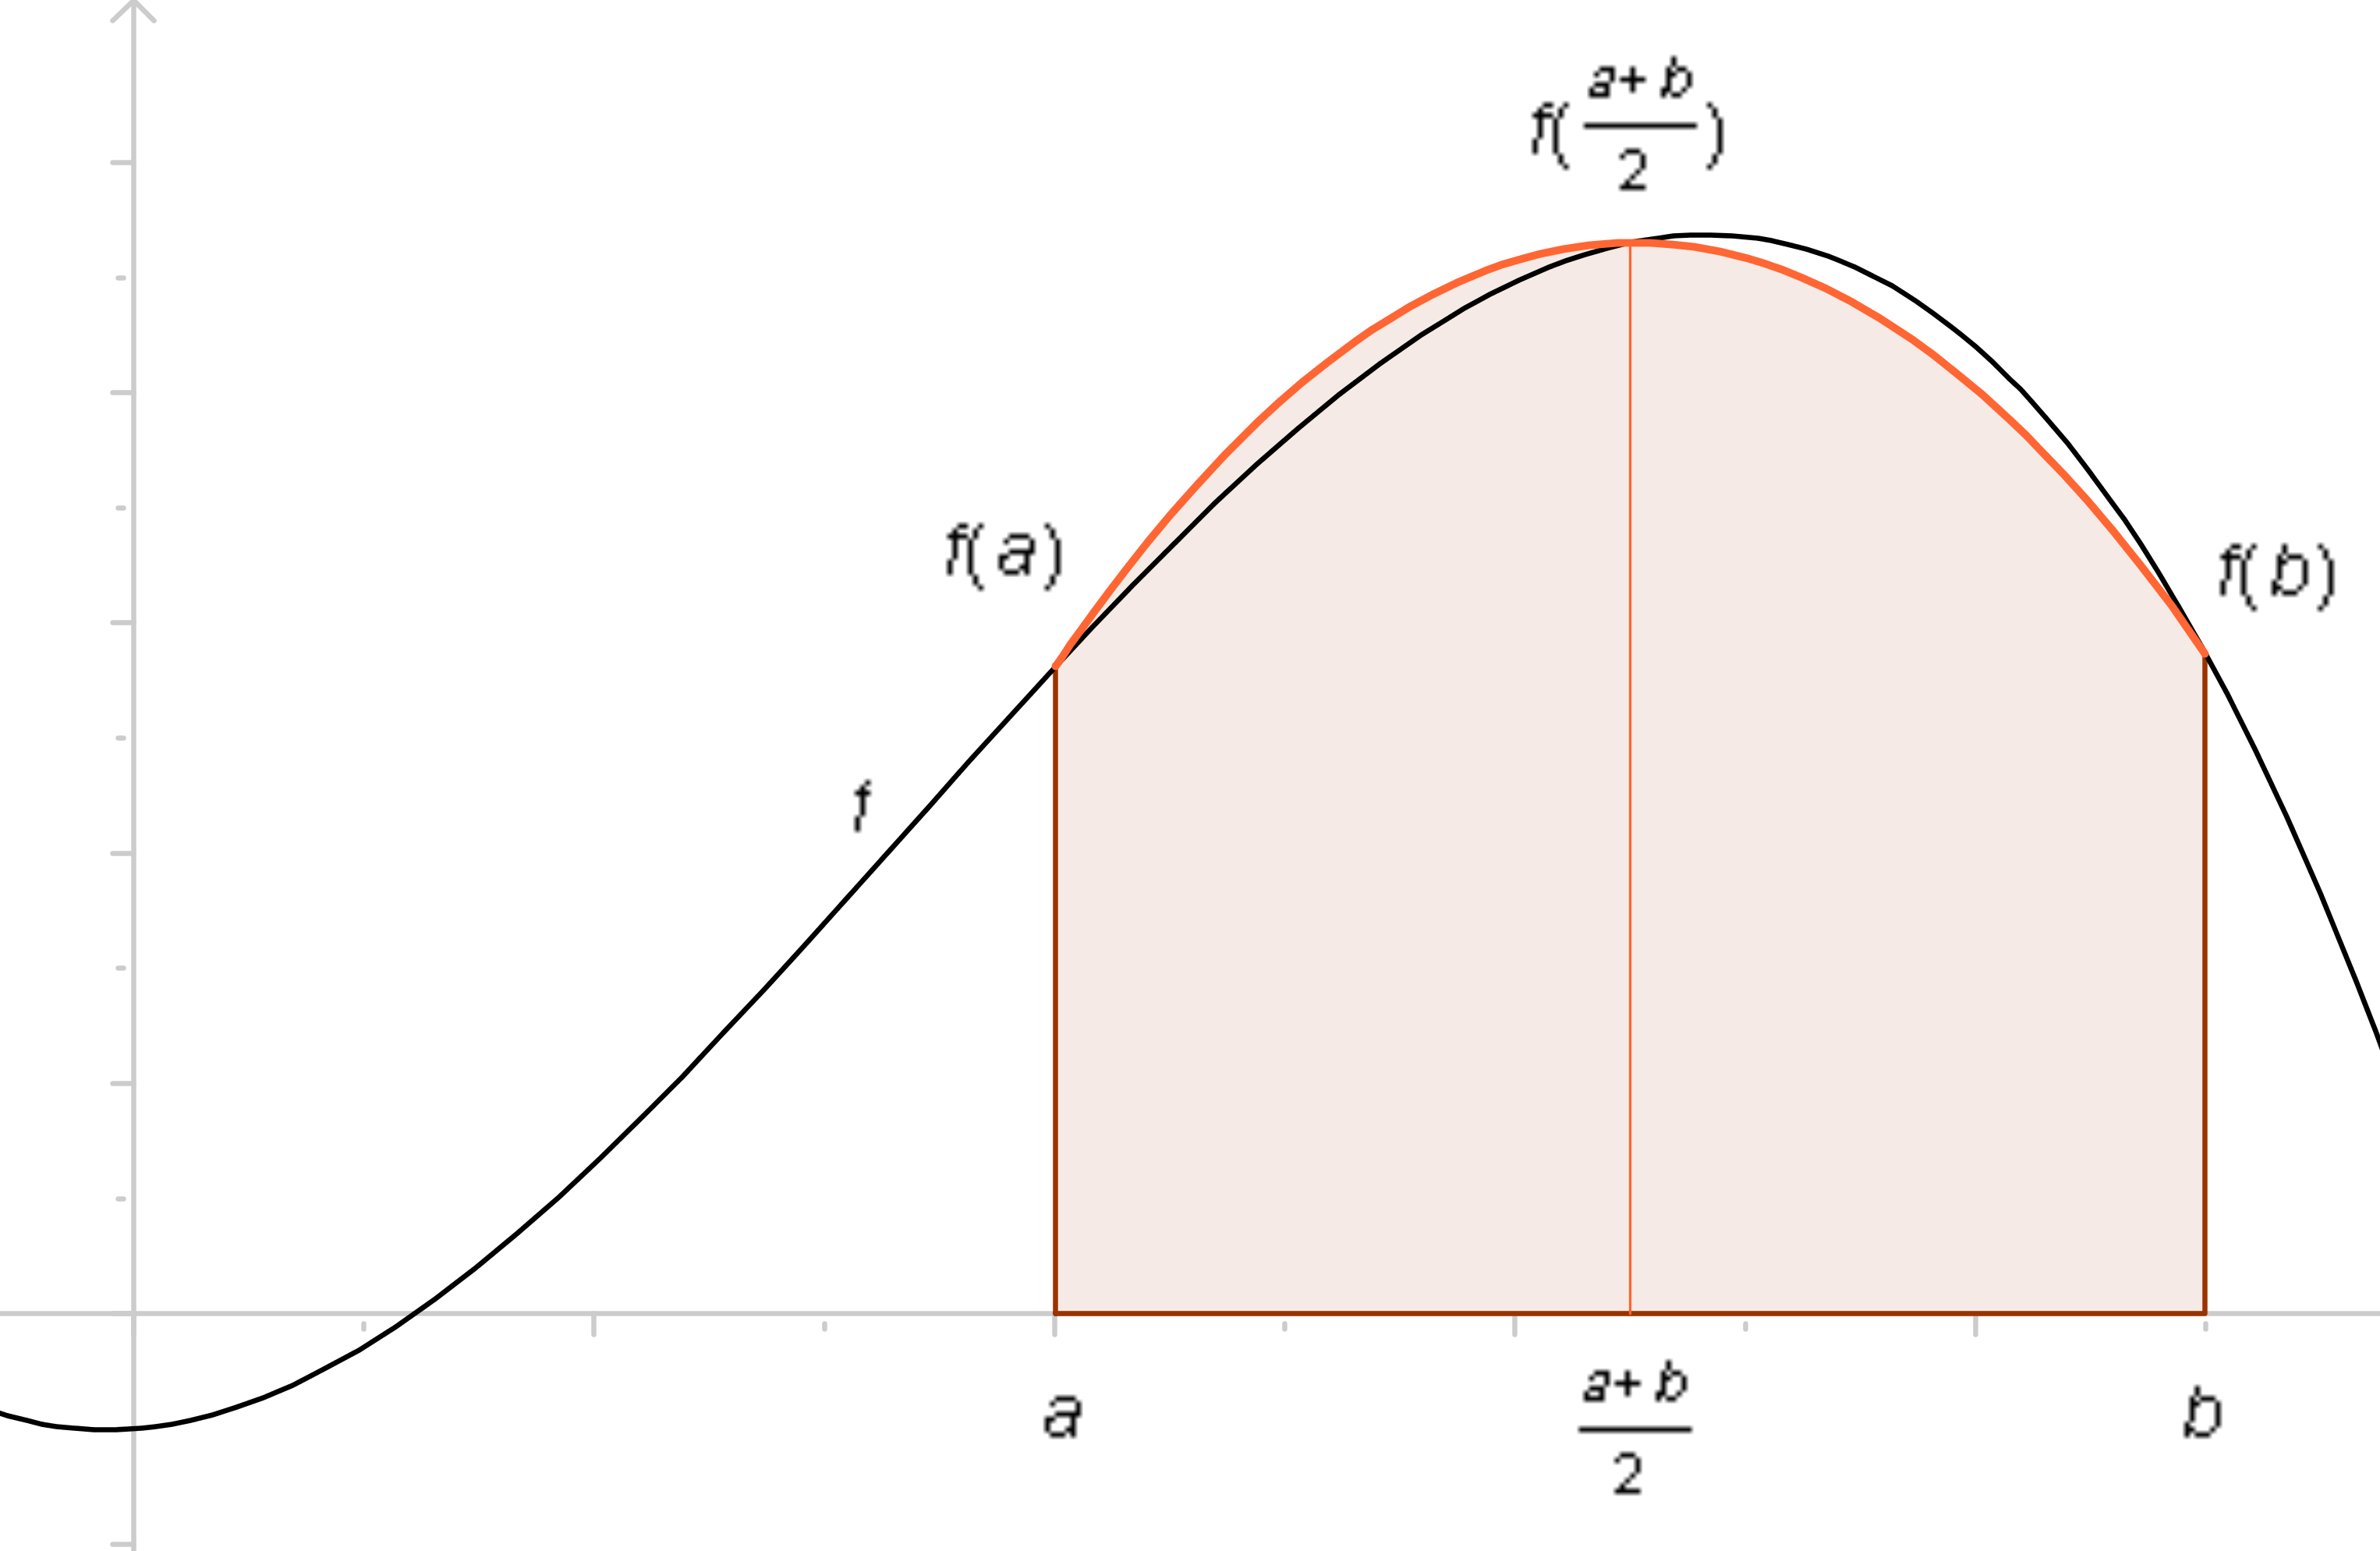
\includegraphics[width=1.5in]{SimpsonRule.png}
\end{center}
\end{frame}

\begin{frame}[fragile]
{\bf Numerical Integration Error Bounds}
Last week we talked a great deal about errors and how important it is for computational scientists to understand the error caused by their mathematical models. 
\vfill \pause
We studied that error is equal to approximate value minus true value. Therefore, in other to determine the error of our numerical integration method, we can simply look at the difference between our result and the true result acquired via exact integration. That's easy! 
\vfill \pause
However, if we are able to get the true value, then why are we bothering with the approximation? \\
\end{frame}

\begin{frame}[fragile]
{\bf Numerical Integration Error Bounds}
\emph{Error bounds} are quantities we can easily compute and are set as ceilings for our errors, that is, the error obtained by a certain mathematical model is guaranteed to be \emph{less} than its error bound. As you might have already guessed, an error bound depends on the mathematical model used (there is no universal error bound).
\vfill \pause
Below are the error bounds for the three methods of numerical integration we've discussed in this lecture.
\end{frame}

\begin{frame}[fragile]
{\bf Numerical Integration Error Bounds}
Let $f$ be the function we are numerically integrating. Suppose that $\max\limits_{a \leq x \leq b}|f''(x)| = K$ and $\max\limits_{a \leq x \leq b}|f^{(4)}(x)| = M$ for $a \leq x \leq b$, then:
\vfill \pause
\begin{enumerate}
\item \emph{The error bound for Midpoint Rule is}
\[\frac{K(b-a)^3}{24n^2}\] \pause
\item \emph{The error bound for Trapezoidal Rule is}
\[\frac{K(b-a)^3}{12n^2}\] \pause
\item \emph{The error bound for Simpson's Rule is}
\[\frac{M(b-a)^5}{180n^4}\]
\end{enumerate}
\end{frame}


\section{An Example: The Error Function}
\begin{frame}[fragile]
{\bf The Error Function}
\[\textnormal{erf}(x) = \frac{2}{\sqrt{\pi}}\int\limits_0^xe^{-t^2}dt\]
The error function (occurring in statistics to measure the behavior of a sample with respect to the population mean) given above is an example of a non-elementary function.
\vfill \pause
Thus it must be expressed as an integral, and if we desire to evaluate erf($x_0$), then we must evaluate the integral that defines erf in the interval $[0,x_0]$.
\vfill \pause
However, this integral has no analytic solution...
\end{frame}

\begin{frame}
{\bf Save us, Julia!}
Let's use IJulia to implement the erf function using the midpoint rule. Our function will take two inputs: the upper bound $x$ of the interval of integration, and the number of sub-intervals $n$.\\
\end{frame}

\begin{frame}[fragile]
{\bf Solution} 
\begin{lstlisting}
# erf's integrand
function integrand(t)
    e^(-t^2)
end    

# erf function using the midpoint rule
function middle_erf(x, n)

    delta_x = x / n
    result = 0
    # summing up the are of rectangles
    for i = 1:n
        x_mid = ((i-1)*delta_x + i*delta_x)/2
        result += delta_x*integrand(x_mid)
    end
\end{lstlisting}
\end{frame}

\begin{frame}[fragile]
{\bf Solution cont.} 
\begin{lstlisting}
    result *= 2 / sqrt(pi)
    
    # since the SECOND derivative of e^(-t^2) is (4t^2 - 2)*(e^(-t^2)),
    # and since it obtains a maximum at t = sqrt(3/2) on the interval 
    # from 0 to x, when x >= sqrt(3/2), OR just at t = x, when 
    # x < sqrt(3/2), then our K in the error bound formula is:
    if x >= sqrt(3/2)
      error_bound = (4/e^(3/2))*(x^3)/(24*n^2)
    else 
      error_bound = abs((4*x^2 - 2)*(e^(-x^2)))*(x^3)/(24*n^2)
    end    
\end{lstlisting}
\end{frame}

\begin{frame}[fragile]
{\bf Solution cont.} 
\begin{lstlisting}
    return ["result" => result, "error bound" => error_bound]
end
\end{lstlisting}
\end{frame}

\end{document}